\documentclass[preprint,12pt]{article}

\usepackage{algorithmic}
\usepackage{algorithm}
\usepackage{enumerate}
\usepackage{enumitem}
\usepackage{graphics}
\usepackage{graphicx}
\usepackage{geometry}
\usepackage{amsmath}
\usepackage{wrapfig}
\usepackage{subfig}
\usepackage{framed}
\usepackage{color}
\usepackage{soul}
\usepackage{bm}

\usepackage{natbib}
\usepackage{multirow}
\usepackage[T1]{fontenc}
\usepackage[latin9]{inputenc}
%\usepackage{units}
\usepackage{esint}
\geometry{legalpaper,  margin=1in}

\newcommand{\CM}[2][green]{ {\sethlcolor{#1} \hl{#2}} }
\newcommand{\KB}[2][cyan]{ {\sethlcolor{#1} \hl{#2}} }
%THIS IS TO PUT ALL FLOATS AT THE END OF THE DOC SO THEY CAN BE SPLIT INTO A SEPARATE FILE
%%\usepackage{endfloat}
%\makeatother

%\usepackage{babel}

\begin{document}
\title{A Bayesian method for Assessing the Extent and Durability of Partisan Gerrymanders}

\author{Kevin Baas and Colin McAuliffe}

\maketitle

\begin{abstract}
We make three improvements to our 2-level Beta model of election outcomes, introduced in a previous paper.  1) We incorporate incumbency effects. 2) We use the Markov Chain Monte Carlo method to impose an implicit prior on the Beta distribution parameters without having to explicitly model the conjugate prior, and 3) We expand the Beta model, which really represents a prior distribution, to a proper posterior predictive distribution, namely, a Beta-Gamma-Binomial distribution.  

After outlining these three improvements, we use the improved model to analyze U.S. House districts for the 2011-2021 redistricting cycle.  We then perform the same analysis on a couple of alternative redistricting algorithms.

We find that the current official method for redistricting (hand-drawn) produces the least representative and least responsive outcomes of all those considered.  Conversely, heuristic optimization produces the most representative and responsive outcomes.  We also find that multi-member districts produce far more representative and responsive outcomes than their single-member counterparts.

In addition to suggesting a way forward for creating more representative and responsive electoral districts, the methods we outline in our paper provide a way to do a comprehensive analysis of the partisan impact of any proposed redistricting plan.  Because it is a Bayesian model, it produces complete likelihood curves, as opposed to a single point estimate.  This gives both legislative and judicial reviewers a more complete picture of the impact of the plan, including a picture of the durability of the effects.

Keywords: Redistricting, gerrymander, modeling

\end{abstract}

\clearpage

\section{Table of symbols}

Throughout the paper, we will use the following symbols as shorthand for denoting their respective quantities:


\begin{tabular}{ll}
\textbf{Symbol} & \textbf{Meaning}                                        \\
d               & district                                                \\
e               & election                                                \\
p               & political party                                         \\
s               & the incumbency effect strength                          \\
popular(e)      & the total popular vote in election e                    \\
vote(d,e)       & the actual vote in district d, election e                   \\
avg()           & the average value taken over all elections in the cycle \\
i(d,e)          & who the incumbent is in district d, election e          \\
f(d,e,s)               & incumbency effect function                              \\
PVI(d)          & the incumbency-neutral PVI for district d                                   \\
aPVI(d,i(d,e))       & the incumbency-boosted PVI for district d, election e   
\end{tabular}


\section{Introduction}

In a previous paper [cite] we introduced a Bayesian probability model for assessing likelihoods of all possible election outcomes.  Our model accounts for the covariance among individual districts by modeling the total popular vote in addition to the individual district votes.   In this model, we used empirical data to:
 
\begin{enumerate}
\item Estimate a Beta distribution for the popular vote,
\item Multiplicatively adjust the per district votes to produce a centered (50-50) popular vote.
\begin{equation}
vote_{centered}(d,e,p) = 
vote(d,e,p) \cdot \frac{ \sum_{d' \in districts}{vote(d',e,p)}}{popular(e,p) } 
\end{equation}

\item Estimate a Beta distribution for each individual district, using these mean-centered vote counts.
\end{enumerate}

This two-layer Beta model is then sampled by:

\begin{enumerate}
\item Sampling from the popular vote Beta distribution
\item Sampling from the individual district Beta distributions
\item Multiplicatively adjusting the individual district results so that the total matches the sampled popular vote.
\end{enumerate}


\begin{equation}
vote_{adjusted}(d,e,p) = 
vote(d,e,p) \cdot \frac{popular(e,p) }{ \sum_{d' \in districts}{vote(d',e,p)}} 
\end{equation}

In this paper we seek to expand on that model to improve its accuracy.  For validation, we compare results from the original simpler model with that of the improved model, by using them both to project election outcomes for the U.S. House.  After that, we use the improved model to generate project election outcomes and likelihood curves for a couple of alternative redistricting algorithms.

\section{Modeling incumbency effects}


\subsection{A saner incumbency effect formula}

Incumbency effect is often modelled as an additive factor on the percent of votes won.  But an incumbency factor of 10 percent added to an initial 95 percent victory results in a 105 percent victory, which is impossible.   In real life, any additive impact on the percentage of votes won due to the incumbency effect drops to zero as the victory margin approaches 100 percent.  To make a more realistic model of the incumbency effect, we need to use a function that does so as well.

\begin{equation}vote_{boosted} = f(vote_{unb
oosted}, s, incumbent)
\end{equation}

\begin{equation}
0 < f(x,s,i) < 1 \forall 0 \le  x \le 1,s,i \in ( -1,0,1)
\end{equation}

As a way to obey this rule, we propose modeling the incumbency effect as a multiplier on expected voter turnout for the incumbent.  This can be interpreted as a vote count boost due to name recognition: more people who turned out to vote will fill in that part of the ballot, because they recognize the name of the incumbent.  An advantage of this function is that it is parsimonious in that it requires no additional free parameters, making it less likely to result in an overfit of the data.  This incumbency effect function can be written formally as:

\begin{equation}
f(x,s,i) = 
\begin{cases}
	\frac{x\cdot s}{ x\cdot s + (1-x)},          & \text{if } i = 1  \\
	x,                                          & \text{if } i = 0  \\
	\frac{1 - (1-x)\cdot s}{ x + (1-x) \cdot s}, & \text{if } i = -1 
\end{cases}
\end{equation}

And its inverse is:

\begin{equation}
f^{-1}(x,s,i) = 
\begin{cases}
	\frac{x\cdot s}{ x / s + (1-x)},          & \text{if } i = 1  \\
	x,                                          & \text{if } i = 0  \\
	\frac{1 - (1-x) / s}{ x + (1-x) / s}, & \text{if } i = -1 
\end{cases}
\end{equation}

\clearpage
\subsection{Estimating incumbency effect strength via neutralization}

We take a statistical regression approach to estimating the effect of incumbency, but first we take a step back and look at the basic idea of statistical regression.  Statistical regression is a method for estimating a parameter by finding a reasonable equation to measure "error", and then developing and applying a method to minimize that error.  The basic method can be summarized like this:

\begin{enumerate}
\item Express error as a function
\item Find the parameter values that minimize that function
\end{enumerate}

For example, in ordinary least squares linear regression, one tries to fit a line to a cloud of points, and the "error" is the sum of squared distances between the line and each point.   The function is squared because this allows us to take derivatives, and thus find the line that produces the exact minimum error by solving an equation.  But the sum of absolute values of differences (called mean absolute deviation) is also a reasonable error function, despite not having a clean analytic solution.  For more complex problems that don't admit analytical solutions, the same general procedure can still be used: express error as a function, then find the parameter values that minimize that function. 

Since we are computing the incumbency parameter in order to use that to improve prediction accuracy, we choose as our "error" function the prediction error that results from using that particular value.  We predict an outcome by adding the incumbency effect to the district's base PVI (partisan voting index).  For the base PVI we simply take the average PVI of all elections ever held in that district.\footnote{Since House elections occur every 2 years, and districts are redrawn every 10 years, that amounts to exactly 5 elections.}

\begin{equation}
PVI(d) = avg(vote(d,e))
\end{equation}

However, since the raw average already includes the incumbency effect, we have to remove the incumbency effect before we calculate the average.

\begin{equation}
PVI(d) = avg(f^{-1}(vote(d,e),s,i(d,e))
\end{equation}

Our predicted result is then this average PVI, with the incumbency effect added in for the incumbent.

\begin{equation}
aPVI(d,i(d,e)) = f(PVI(d),s,i(d,e))
\end{equation}

Finally, our prediction error function is the sum of absolute values of the predicted result minus the actual result:

\begin{equation}
error = \sum_{d, e}{\left| (aPVI(d,i(d,e)) - vote(d,e)\right|}
\end{equation}

Substituting in the formula for aPVI produces:

\begin{equation}
error = \sum_{d,e}{\left|  f(PVI(d),s,i(e)) - vote(d,e)\right|}
\end{equation}

And then substituting in the formulal for PVI produces:

\begin{equation}
error = \sum_{d,e}{\left|  f[ avg(f^{-1}(vote(d,e'),s,i(d,e')) ,s,i(d,e) ] - vote(d,e)\right|}
\end{equation}

This is our error function to minimize.  We then write a computer program to test different values of our incumbency effect parameter, s, from 1.0 to 1.5, in increments of 0.01, and find the value that minimizes this error.  Furthermore, we plot this curve and visually confirm that it has no local minima besides the global minimum, thus confirming that our function is "well-behaved" in the sense that this approach to minimizing it produces a reasonable and reliable solution.

\subsection{Results of incumbency estimation}

Using U.S. House election results for all 50 states, for all elections from 1972 to 2016 (inclusive), collected by Brian Remlinger and Sam Wang, we estimated the incumbency effect strength for each districting cycle.  

In order to obtain vote counts in uncontested races we used an imputation procedure. The two party vote shares in an uncontested district are taken as the average of the vote shares for that district in the same cycle. If a district is uncontested for an entire election cycle, then the vote share is taken to be equal to the average of the most partisan district for the winning party. The voter turnout in the uncontested district is then taken as the average turnout in all contested elections in that state and election year. Generally it is preferable to impute uncontested results using presidential results at the district level, but such data was not available for the entire time period under study. Like all methods for examining gerrymandering, the specific asymmetry and the Bayesian simulation method are sensitive to the particular imputation technique employed, although a comprehensive study of this sensitivity is beyond the scope of our present work.

\begin{figure}[htb!]
    \begin{center}
        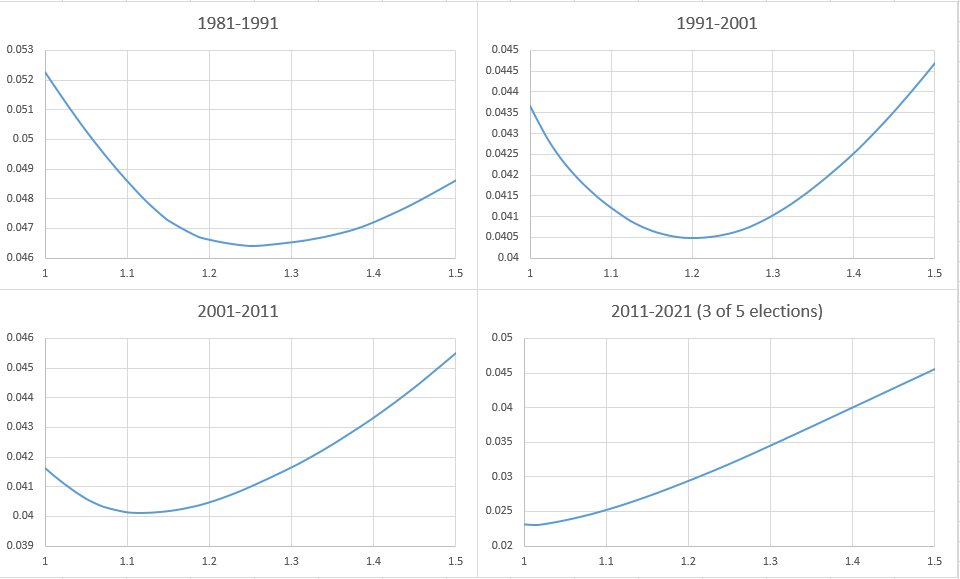
\includegraphics[scale=0.5]{Figures/incumbency.png}
        \caption{Prediction error as a function of incumbency effect strength}\label{fig:incumbency}
    \end{center}
\end{figure}

We found that the following turnout multipliers minimized prediction error for the corresponding cycles:

\begin{itemize}
\item 1981-1991: 1.25
\item 1991-2001: 1.20
\item 2001-2011: 1.11
\item 2011-2021 (partial): 1.01
\end{itemize}

For the 2011-2021 cycle, we only had three elections to predict, instead of the usual five.  This may account for the lower estimated incumbency effect strength.  In all cases, the error function is roughly parabolic, suggesting that the minima are robust and global.

Additionally we considered the possibility that the strength of the incumbency effect is different for each party, and the possibility that it's different in election years with a presidential election, verses years without (midterms).  To assess how strong these potential differences are, we calculated the average prediction error resulting from 3 different methods of accounting for incumbency, versus not accounting for incumbency at all.  We found that that average absolute prediction error:

\begin{itemize}
\item without the incumbency effect was 4.00 percent, 
\item adding a single parameter incumbency effect reduced that to 3.66 percent, 
\item using separate strengths for presidential and midterm elections reduced that by less than 0.0015 percent
\item using separate incumbency strengths for democrats and republicans reduced that even less
\end{itemize}

From this we conclude that the potential for improvement by using two different incumbency effect strengths along either of these lines is negligible, at best.  

This disagrees with various analysis done by others [cite a few].  We suspect that the other authors accidently over-fit the data; that the sample size they used was not sufficient to support their conclusions. However, without a thorough analysis of the data, we can do little more than speculate.

Regardless, for the sake of this study, we've determined that the predictive power of the additional parameter does not mathematically justify its use, and indeed, justifies its non-use.  We have therefore deliberately chosen to stick with a single incumbency strength for all parties, and all election years in a redistricting cycle.

\subsection{Adding incumbency effect to the 2-level Beta model}

Recall the steps to generate our 2-level Beta model:

\begin{enumerate}
\item Estimate a Beta distribution for the popular vote,
\item Multiplicatively adjust the per district votes to produce a centered (50-50) popular vote.
\item Estimate a Beta distribution for each individual district, using these mean-centered vote counts.
\end{enumerate}

To incorporate the incumbency effect into this model, we simply insert two steps to the beginning of this process:

\begin{enumerate}
\item Apply the divide the vote counts of challenged incumbents by the incumbency effect strength, to neutralize it.
\item (optionally) Multiply the resulting vote counts of challenged incumbents in the election to be projected by the incumbency effect strength.
\end{enumerate}

And then proceed as usual through the original steps.  In other words, accounting for incumbency can be viewed as a "pre-processing" step.  We refer to procedures that apply step one but not step two as "incumbency neutral" models.

\section{Using MCMC to do Bayesian estimation of the Beta parameters}

\section{A more complete model (a proper posterior predictive) beta-binomial with gamma estimation of n}

\section{Visualizing the outcomes}

Using a Bayesian model enables us to calculate complete likelihood curves, as opposed to just point estimates, for any quantity that we can formally describe.  These likelihood curves can be generated by sampling the posterior predictive distribution, and then applying the formula for the measured quantity to the samples.  For consistency and ease of comparison, in each of our analysis, we will compute likelihoods curves for the same four measures.  The measures were chosen with the intention that, taken together, they will give a complete picture of the electoral consequences of the redistricting plan.



The first measure we refer to informally as a "total view", and more formally as a seats-votes heatmap. This is a 3-dimensional chart showing on one axis a potential popular vote fraction, on another axis a potential seat count, and on the third, the probability of that combination.  So the function being graphed is z = p( vote percent, seat count). "z" is represented by color saturation (darkness).  In this way, the chart resembles a "heat map". We call this the "total view" because all other charts we present can be derived from this one.

(Sample image)

From this, we get a likelihood of either party winning the majority of seats, simply by totaling the volume in each half of the chart. 

(Sample image)

Additionally we measure representation and responsiveness.  Representation is how much the outcome reflects the will of the voters.  Responsiveness is how much the outcome changes when voter preferences change.  It's important to note that these two components are independent of each other.  Roughly speaking, responsiveness is the first derivative of representation; responsiveness is to representation as speed is to distance.

Single-winner elections can't produce linearly proportional results, but instead produce a sigmoidal seats-votes curve.  To account for this, we use specific asymmetry to measure representation instead of deviation from a diagonal line.  This tells us how much of a party's excess seat gain is due to gerrymandering, as opposed to an inevitable consequence of  the sigmoidal nature of the seats-votes curve.  This can be extracted from the "total view" by comparing each point on the total view with its two-axis reflection.  The vertical distance between a point and it's reflection represents the specific asymmetry, and the color saturation represents the likelihood of that outcome.  These likelihoods are totalled up for every possible value of the specific asymmetry, and graphed on a chart where y represents likelihood and x represents specific asymmetry.

(Sample image)

We measure responsiveness as the first derivative of representation; as the change in seat count per change in vote share.   The visual slope of the "total view" gives a quick sense of the responsiveness, but it is not so straightforward to translate this into a quantitative likelihood curve.  Each point on the total view represents millions of different possible scenarios.  And for each of those different scenarios, a different change in the popular vote balance is needed to change the seat count. 

So instead we go back to the raw potential outcomes.  For each potential outcome, we calculate how much the popular vote needs to change to add a democratic seat, and how much the popular vote needs to change to add a republican seat.  We then graph each of these separately on a chart, with the x axis representing fraction of popular vote change for the next seat, and the y axis representing cumulative likelihood.

(Sample image)

In conclusion, we will produce 4 charts to assess the partisan impact of each redistricting plan that we analyze: a seats-votes likelihood curve, a bar chart of likelihood to win the majority, a likelihood chart of specific asymmetry, and a cumulative likelihood chart of votes needed to win the next seat.  The charts will be arranged in a 2x2 grid like so:


\section{A projection of the U.S. House using the improved model}
(compare 2x2 - incumbency, no incumbency, and original beta model, beta-gamma-binomial)
(do two decades: 2000 and 2010)

In order to see if our changes to the Bayesian probabiliy model produce a posterior predictive distribution that more closely matches the true distribution, we use both the original model and the augmented model to project likelihoods for the U.S. House, and compare the results. If our augmented model is better, we should expect to see similiar results, with somewhat increased variance, but not excessively increased variance.  If we do leave-one-out-validation, we should see slightly higher log-likelihood in the augmented model.


\section{What the U.S. House would be like under alternative districting algorithms}

We used presidential election data from 2004, 2008, and 2012 elections, at voting ward resolution, from Stephen Wolf of DailyKo's Google drive.  We then used AutoRedistrict to design heuristically optimized districts for all 50 states, for single member and multi-member proportional districts, both for the current 435 seat count and a theoretically expanded seat count of 593.  To this we added the current actual districts, the previous census cycle's districts, and compactness-optimized districts created using BDistricting.   We then used AutoRedistrict to combine the district shapes with the ward-resolution election vote counts, and export district-resolution election vote counts, for all 3 elections.

We then used our 2-level Beta-Gamma-Binomial model to compute likelihoods curves for each of these redistricting methods. 

These methods can also be applied at state and local levels (e.g. state legislative, city council), and on different types of districts (e.g. police districts, voting wards)

\begin{figure}[htb!]
    \begin{center}
        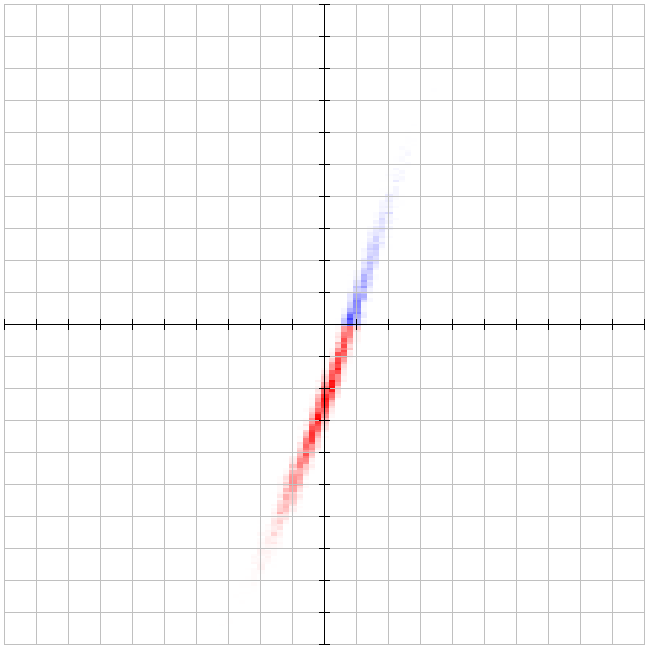
\includegraphics[scale=0.5]{Figures/original_method/2010_ush.png}
        \caption{2010 U.S. House districts, seats-votes likelhoods}\label{fig:2010_ush}
    \end{center}
\end{figure}
\begin{figure}[htb!]
    \begin{center}
        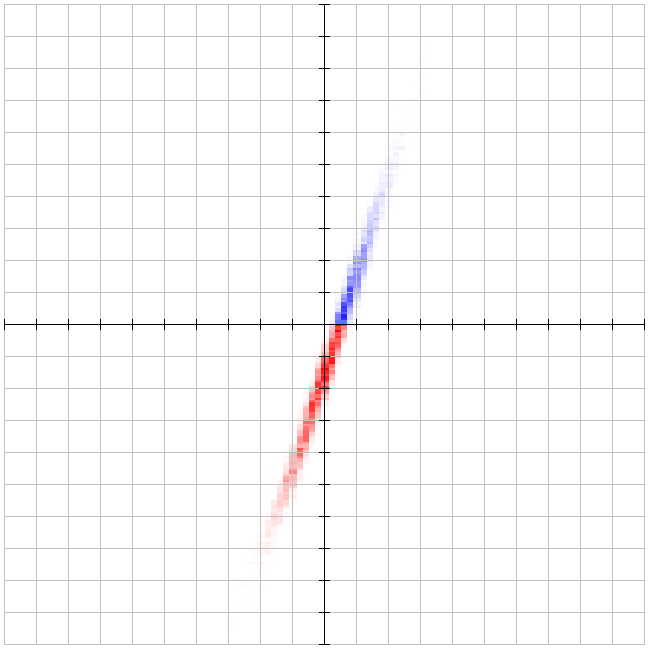
\includegraphics[scale=0.5]{Figures/original_method/2000_ush.png}
        \caption{2000 U.S. House districts, seats-votes likelhoods}\label{fig:2000_ush}
    \end{center}
\end{figure}
\begin{figure}[htb!]
    \begin{center}
        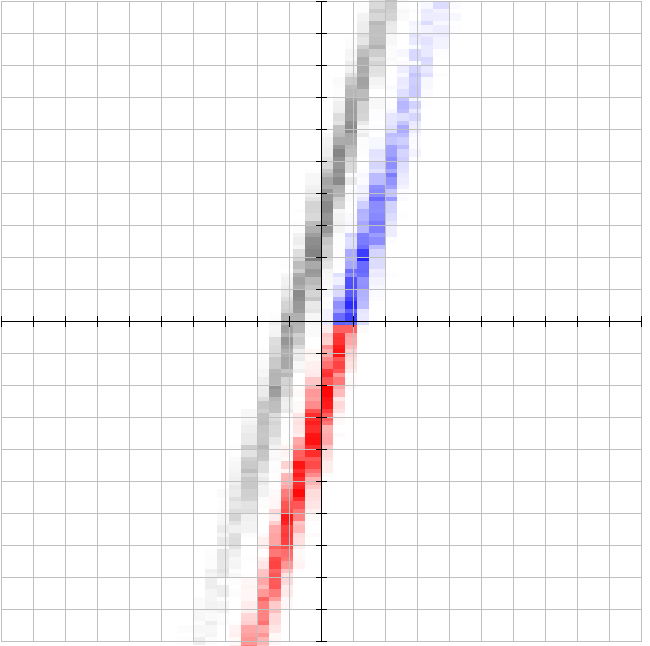
\includegraphics[scale=0.5]{Figures/original_method/BD__ush.png}
        \caption{Compactness optimized U.S. House districts, seats-votes likelhoods}\label{fig:BD_ush}
    \end{center}
\end{figure}
\begin{figure}[htb!]
    \begin{center}
        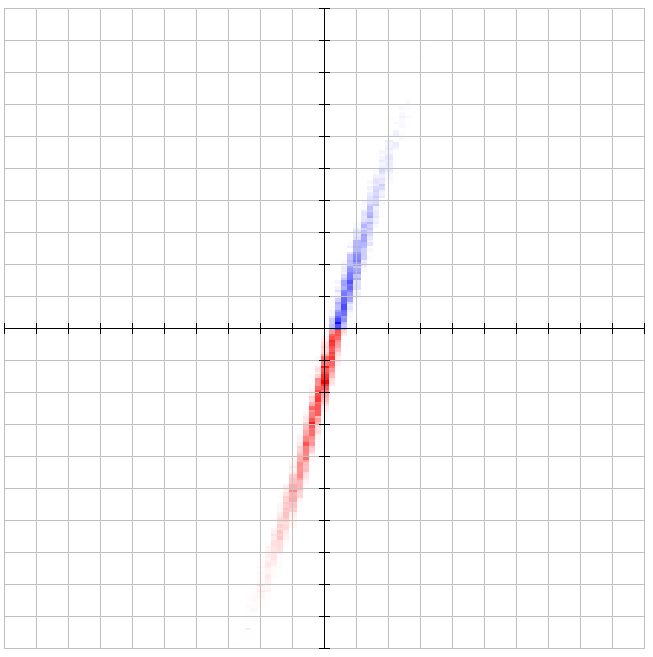
\includegraphics[scale=0.5]{Figures/original_method/SM__ush.png}
        \caption{Multi-objective optimized U.S. House districts, seats-votes likelhioods}\label{fig:SM_ush}
    \end{center}
\end{figure}
\begin{figure}[htb!]
    \begin{center}
        \includegraphics[scale=0.5]{Figures/original_method/fv_ush.png}
        \caption{Multi-member proportional U.S. House districts, seats-votes likelhioods}\label{fig:SM_ush}
    \end{center}
\end{figure}

Our results indicate that in the 2010 redistricting cycle, Republicans systematically gerrymandered the U.S. House, giving Democratic voters a large structural disadvantage. The popular vote would have to favor Democrats by more than an 8 percent margin, just to give them a majority of seats.  This contrasts sharply with what seats-votes likelihoods would be like if elections were still held under the districts from the 2000-cycle redistricting.  If the partisan gerrymandering in 2010 did not occur, Democratic voters would only have to win the popular vote by a little over 5 percent margin in order to get half of the U.S. house seats.

If instead all states in the country used an algorithm to optimize compactness of districts, the result would be about the same.  This suggests that most of the gerrymandering in the 2000-cycle was accidental; that it was due to political self-sorting, as opposed to deliberate gerrymandering.  If instead all states in the country used an alogirhtm that also minimized seats-votes curve asymmetry, the amount of partisan gerrymandering would be further reduced, and Democrats would only have to win the popular vote by a 3 percent margin in order to win the majority of seats.

Finally, using multi-member proportional districts appears to completely eliminate partisan gerrymandering, in addition to making the seat allocations more proportional and more responsive to changes in voter sentiment.  Our nation-wide statistical analysis of alternative redistricting algorithms suggests that, when it comes to representation and responsiveness, the voting and tallying system is far more important than the redistricting algoorithm.  In other words, if the goal is to eliminate gerrymandering and make elections more responsive, then instead of focusing on how changes to the redistricting process can reduce or eliminate gerrymandering, we should be focused on a fundamental overhaul on how congressional seats are assigned.

Taken together, these results appear to indicate that automated redistricting provides more partisanly fair results than manually-drawn maps, regardless of the algorithm used.  Our results further show that compactness-only algorithms still leave a substantial amount of partisan gerrymandering, which gives a large class of voters (roughly half the country) a systematic structural disadvantage to representation.  This harm can be reduced substantially by including a partisan-symmetry criteria in the optimization algorithm, and it can be almost completely eliminated by using multi-member proportional districts.  Furhtermore, multi-member proportional districts are more responsive to changes in voter sentiment, and produce more proportional representation.

\section{Conclusion}

We made three separate improvements to our Bayesian Empirical model of election result likelihoods that we presented in a previous paper.  We then tested the efficacy of these improvements using historical U.S. House election returns.  We found that, measured in log-likelihood of actual returns, our changes led to a slight improvement in accuracy.  Finally, we used this probability model to project outcome likelihoods for various alternative redistricting algorithms, and analyze these likelihoods in four different ways.

We found that the current official method for redistricting (hand-drawn) produces the least representative and least responsive outcomes of all those considered.  Conversely, heuristic optimization produces the most representative and responsive outcomes.  We also found that multi-member districts produce far more representative and responsive outcomes than their single-member counterparts.

More importantly, the methods we've developed and outlined can be used by independent election commisions to assess the impact of potential district designs, and by plaintiffs to contest those designs on account of their impact.



\clearpage

\end{document}
